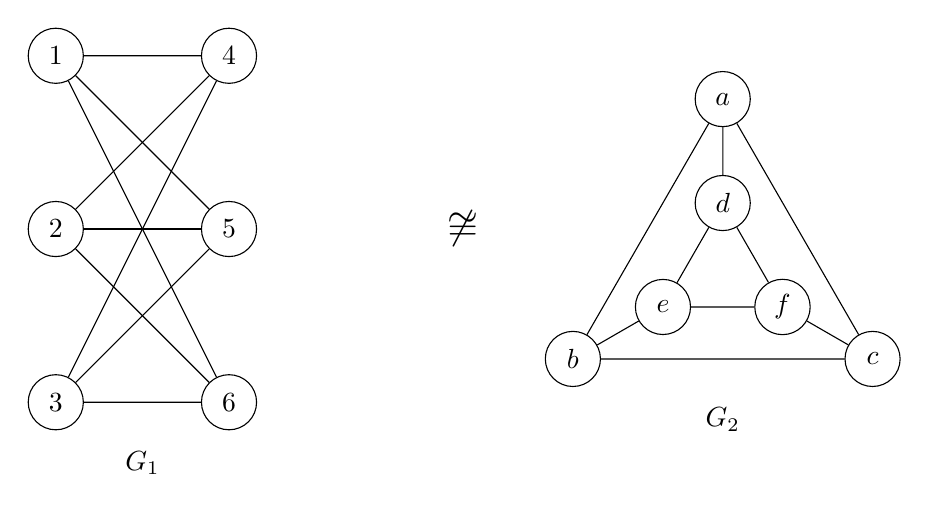
\begin{tikzpicture}[
    scale=1.1,
    every node/.style={circle, draw, minimum size=7mm}
]


% ================= G1 : K_{3,3} =================

\node (v1) at (-0.7,2)  {$1$};
\node (v2) at (-0.7,0)  {$2$};
\node (v3) at (-0.7,-2) {$3$};

\node (v4) at (1.3,2)   {$4$};
\node (v5) at (1.3,0)   {$5$};
\node (v6) at (1.3,-2)  {$6$};

\draw (v1)--(v4);
\draw (v1)--(v5);
\draw (v1)--(v6);

\draw (v2)--(v4);
\draw (v2)--(v5);
\draw (v2)--(v6);

\draw (v3)--(v4);
\draw (v3)--(v5);
\draw (v3)--(v6);

\node[draw=none, rectangle] at (0.3,-2.7) {$G_1$};

% ================= G2 : prisme triangulaire (recentré sur y=0) =================

\node (ua) at (7,1.5)     {$a$};
\node (ub) at (5.27,-1.5) {$b$};
\node (uc) at (8.73,-1.5) {$c$};
\node (ud) at (7,0.3)     {$d$};
\node (ue) at (6.31,-0.9) {$e$};
\node (uf) at (7.69,-0.9) {$f$};

\draw (ua)--(ub);
\draw (ub)--(uc);
\draw (uc)--(ua);
\draw (ud)--(ue);
\draw (ue)--(uf);
\draw (uf)--(ud);
\draw (ua)--(ud);
\draw (ub)--(ue);
\draw (uc)--(uf);

\node[draw=none, rectangle] at (7,-2.2) {$G_2$};

% ================= Symbole de non-isomorphisme =================

\node[draw=none, rectangle] at (4,0) {\Large $\not\cong$};

\end{tikzpicture}